\documentclass[spanish, fleqn]{article}
\usepackage{babel}
\usepackage[utf8]{inputenc}
\usepackage{amsmath}
\usepackage{amsfonts}
\usepackage[colorlinks, urlcolor=blue]{hyperref}
\usepackage{fourier}
\usepackage{tikz}
\usepackage[top = 2.5cm, bottom = 2cm, left = 2cm, right = 2cm]{geometry}

\usetikzlibrary{automata, arrows, positioning, babel}
\tikzset{shorten >= 1pt,
	 node distance = 1.8cm, on grid,
	 >= stealth,
	 initial text = Inicio,
	 every state/.style = {draw, very thick,
			       minimum size = 5mm},
	 bend angle = 35,
	 every loop/.style = {looseness = 13}}

\newcommand{\num}{1}

\title{Informática Teórica\\
       Tarea \#\num \\
       ``Esto no se compila''}
\author{Andrés Navarro // 201673001-K}
\date{25 de septiembre de 2017}

\begin{document}
\maketitle
\pagestyle{empty}
\thispagestyle{empty}

  Una forma alternativa de construir una expresión regular
  que reconoce el lenguaje aceptado
  por el DFA \(M = (Q, \Sigma, \delta, q_0, F)\)
  es plantear expresiones regulares
  para las palabras que llevan al DFA desde el estado inicial
  a cada uno de los estados.
  Básicamente,
  llamando \(R_q\) a la expresión para llegar al estado \(q\),
  si \(\delta(q, a) = p\),
  entre las alternativas para \(R_p\) estará \(R_q a\).
  El lenguaje aceptado por \(M\) es la alternancia entre las expresiones
  para estados finales.

  Esto termina en un sistema de ecuaciones para los distintos \(R_q\),
  podemos usar nuestro teorema
  sobre solución de ecuaciones de la forma \(X = X A \cup B\) entre lenguajes
  para resolver una de ellas,
  y substituir en las demás,
  hasta finalmente tener todos los \(R_q\) requeridos.

  Comentarios en C++ quedan definidos
  por el DFA de la figura~\ref{fig:20172t2},
  donde hemos omitido el estado muerto
  y las transiciones a él para simplificar.
  El alfabeto usado es \(\{ /, *, a, n \}\),
  donde \(/\) y \(*\) representan esos caracteres,
  \(n\) representa al fin de línea
  (se escribe \('\backslash n'\) en C++)
  y \(a\) es cualquier otro caracter válido.
  \begin{figure}[ht]
    \centering
    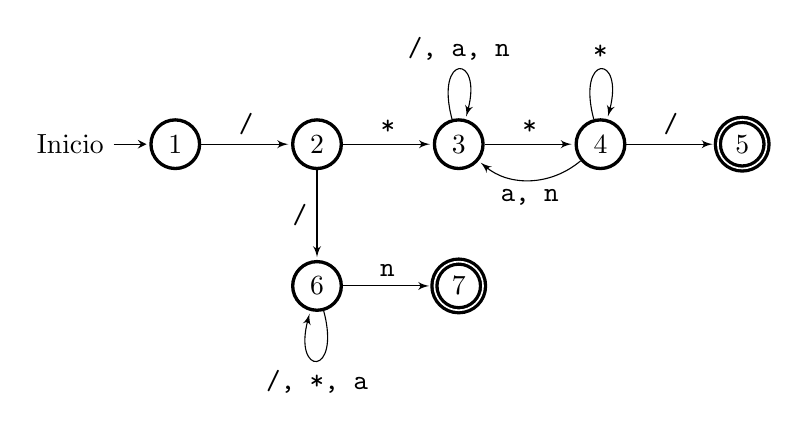
\begin{tikzpicture}
      \node [initial, state] (1) {1};
      \node [state] (2) [right of = 1] {2};
      \node [state] (3) [right of = 2] {3};
      \node [state] (4) [right of = 3] {4};
      \node [state, accepting] (5) [right of = 4] {5};
      \node [state] (6) [below of = 2] {6};
      \node [state, accepting] (7) [right of = 6] {7};
      \path[-latex'] (1) edge [above] node {\texttt{/}} (2)
		     (2) edge [above] node {\texttt{*}} (3)
		     (2) edge [left]  node {\texttt{/}} (6)
		     (3) edge [above] node {\texttt{*}} (4)
		     (4) edge [above] node {\texttt{/}} (5);
      \path[-latex'] (3) edge [loop above] node {\texttt{/, a, n}} ()
		     (4) edge [loop above] node {\texttt{*}} ();
      \path[-latex'] (4) edge [bend left = 40] node[below]
				 {\texttt{a, n}} (3);
      \path[-latex'] (6) edge [loop below] node {\texttt{/, *, a}} ()
		     (6) edge [above] node {\texttt{n}} (7);
    \end{tikzpicture}
    \caption{Comentarios en C++}
    \label{fig:20172t2}
  \end{figure}
  \begin{enumerate}
  \item % 20172t2p1
    Plantee el sistema de ecuaciones descrito
    para expresiones regulares \(R_1\) a \(R_7\)
    partiendo del autómata de la figura~\ref{fig:20172t2}.
    Use \(s\) en vez del símbolo \(*\) para evitar ambigüedades.
    
    Dado que $R_{1}$ es el correspondiente al estado $1$, el cual es el inicial, se llega a el consumiendo solamente $\epsilon$, para el resto de expresiones $R_{n}$, su ecuación fue confecionada visualizando el autómata. 
    \begin{align*}
    R_{1}&=\epsilon \\
    R_{2}&=R_{1}/\\
    R_{3}&=R_{2}s|R_{3}/|R_{3}a|R_{3}n|R_{4}a|R_{4}n\\
    R_{4}&=R_{3}s|R_{4}s\\
    R_{5}&=R_{4}/\\
    R_{6}&=R_{2}/|R_{6}/|R{6}s|R_{6}a\\
    R_{7}&=R_{6}n\\
    \end{align*}
    
    
  \item % 20172t2p2
    \label{ques:20172t2p2}
    Dé la expresión regular para el lenguaje aceptado por el autómata
    en términos de los \(R_k\).
    
  \item % 20172p2t3
    Indique paso a paso cómo resuelve el sistema de ecuaciones
    para las variables necesarias para la pregunta~\ref{ques:20172t2p2}.
    
    Primero reemplazamos $R_{1}$ en $R_{2}$
    \begin{align*}
    R_{1}&=\epsilon \\
    R_{2}&=R_{1}/ \Rightarrow R_{2}=\epsilon/ \Rightarrow R_{2}=/
    \end{align*}
    Trabajando sobre $R_3$
    \begin{align*}
    &\text{Primero tenemos:}\\
    &R_3=R_{4}a|R_{4}n \Rightarrow R_3=R_4(a|n)\\
    &\text{Con lo obtenido anteriormente de $R_2$:}\\
    &R_3=R_2s \Rightarrow R_3=/s\\
    &\text{Tenemos:}\\
    &R_3=/s|R_{3}/|R_{3}a|R_{3}n|R_4(a|n) \Rightarrow R_3=/s|R_3(/|a|n)|R_4(a|n) \\
    &\text{Ahora, ocupando el teorema 1.1:}\\
    &R_3=/s|R_3(/|a|n) \Rightarrow R_3=/s(/|a|n)^*\\
    &R_3=R_4(a|n)|R_3(/|n|a) \Rightarrow R_3=R_4(a|n)(/|n|a)^*\\
    &\text{Finalmente:}\\
    &R_3=/s(/|a|n)^*|R_4(a|n)(/|n|a)^*
    \end{align*}
    Trabajando sobre $R_4$
    \begin{align*}
    &\text{Ocupando el teorema 1.1 tenemos:}\\
    &R_4=R_3s|R_4s \Rightarrow R_4=R_3ss^*\\
    &\text{Sabiendo que $ss*=s^+$:}\\
    &R_4=R_3s^+\\
    &\text{Con lo obtenido en $R_3$:}\\
    &R_4=(/s(/|a|n)^*|R_4(a|n)(/|n|a)^*)s^+ \Rightarrow R_4=/s(/|a|n)^*s^+|R_4(a|n)(/|n|a)^*s^+\\
    &\text{Ocupando el teorema 1.1 tenemos:}\\
    &R_4=/s(/|a|n)^*s^+|R_4(a|n)(/|n|a)^*s^+ \Rightarrow R_4=/s(/|a|n)^*s^+((a|n)(/|n|a)^*s^+)^*
    \end{align*}
    Trabajando sobre $R_5$
    \begin{align*}
	&\text{Ocupando lo obtenido en $R_4$:}\\
    &R_5=R_4/ \Rightarrow R_5=/s(/|a|n)^*s^+((a|n)(/|n|a)^*s^+)^*/
    \end{align*}
    Trabajando sobre $R_6$:
    \begin{align*}
	&R_6=R_{6}/|R{6}s|R_{6}a \Rightarrow R_6=R_6(/|s|a)\\
	&\text{Ocupando el teorema 1.1 tenemos:}\\
	&R_6=R_2/|R_6(/|s|a) \Rightarrow R_6=R_2/(/|s|a)*\\
	&\text{Reemplazando $R_2$:}\\
	&R_6=//(/|s|a)*
    \end{align*}
    Trabajando sobre $R_7$:
    \begin{align*}
    &\text{Reemplazando $R_6$:}\\
    &R_7=R_6n \Rightarrow R_7=//(/|s|a)*n
    \end{align*}
  \end{enumerate}

% Condiciones generales de tareas de Fundamentos de Informática I, 2015
\section*{Condiciones Generales}

  \begin{itemize}
  \item
    La tarea se realizará \emph{individualmente}
    (esto es grupos de una persona),
    sin excepciones.
  \item
    La tarea debe ser entregada impresa
\if\num0
\else
     o manuscrita
\fi
    en
    la Secretaría Docente de Informática
    (Piso 1, edificio F3)
    el día indicado en \href{http://moodle.inf.utfsm.cl}{Moodle}.
  \item
\if\num0
    Junto
\else
    Opcionalmente,
    puede desarrollar la tarea en \LaTeX{},
    lo cual tiene una bonificación de 10 puntos.
    Para obtener la bonificación,
    junto
\fi
    con entregar la tarea impresa en hojas tamaño carta
    deberá depositar copia
    de los fuentes \LaTeX{} de su solución en un \emph{tarball}
    en el área designada al efecto
    en \href{http://moodle.inf.utfsm.cl}{Moodle}
    bajo el formato
    \texttt{tarea\num-\emph{rol}.tar.gz}.
    El archivo debe contener el directorio \texttt{tarea\num-\emph{rol}},
    en el cual están los archivos de su solución
    (al menos \texttt{tarea\num.tex}).
\if\num0
    Sólo se considerará entregada correctamente la tarea si
\else
    Tiene derecho a la bonificación sólo si
\fi
    el \emph{tarball} tiene el nombre y contenido correctos,
    y los fuentes \LaTeX{}
    (y posibles otros archivos anexos)
    se procesan correctamente
    en el ambiente que ofrece el Laboratorio de Computación
    del Departamento de Informática,
    y están escritos en forma legible.
\if\num0
\else

    Si la entrega es en manuscrito,
    está afecta a descuento de hasta 20 puntos por desorden o ilegibilidad.
\fi
\ifdefined\ontime
  \item
    El plazo de entrega dado para esta tarea es definitivo,
    no se aceptan entregas atrasadas.
\else
  \item
    Por cada día de atraso se descontarán 20 puntos.
    A partir del tercer día de atraso
    no se reciben más tareas y la nota es automáticamente cero.
\fi
  \item
    La nota de la tarea puede ser según lo entregado,
    o (en el caso de algunos estudiantes elegidos al azar)
    el resultado de una interrogación en que deberá explicar lo entregado.
    No presentarse a la interrogación significa automáticamente
    nota cero.

    Sobre la nota de la interrogación se aplican
\ifdefined\ontime
    la bonificación por entrega en \LaTeX{}
    o el descuento por desorden.
\else
    los descuentos por atraso
    si proceden%
\if\num0%
    .%
\else%
    ,
    y la bonificación por entrega en \LaTeX{}
    o los descuentos por desorden.
\fi
\fi
  \end{itemize}

  \vfill\hfill LW/HvB/\LaTeXe
\end{document}

%%% Local Variables:
%%% mode: latex
%%% TeX-master: t
%%% End:
